\section{Partial Writes in SSD RAID}
\label{sec:partial}

\begin{figure}[t]
\centering
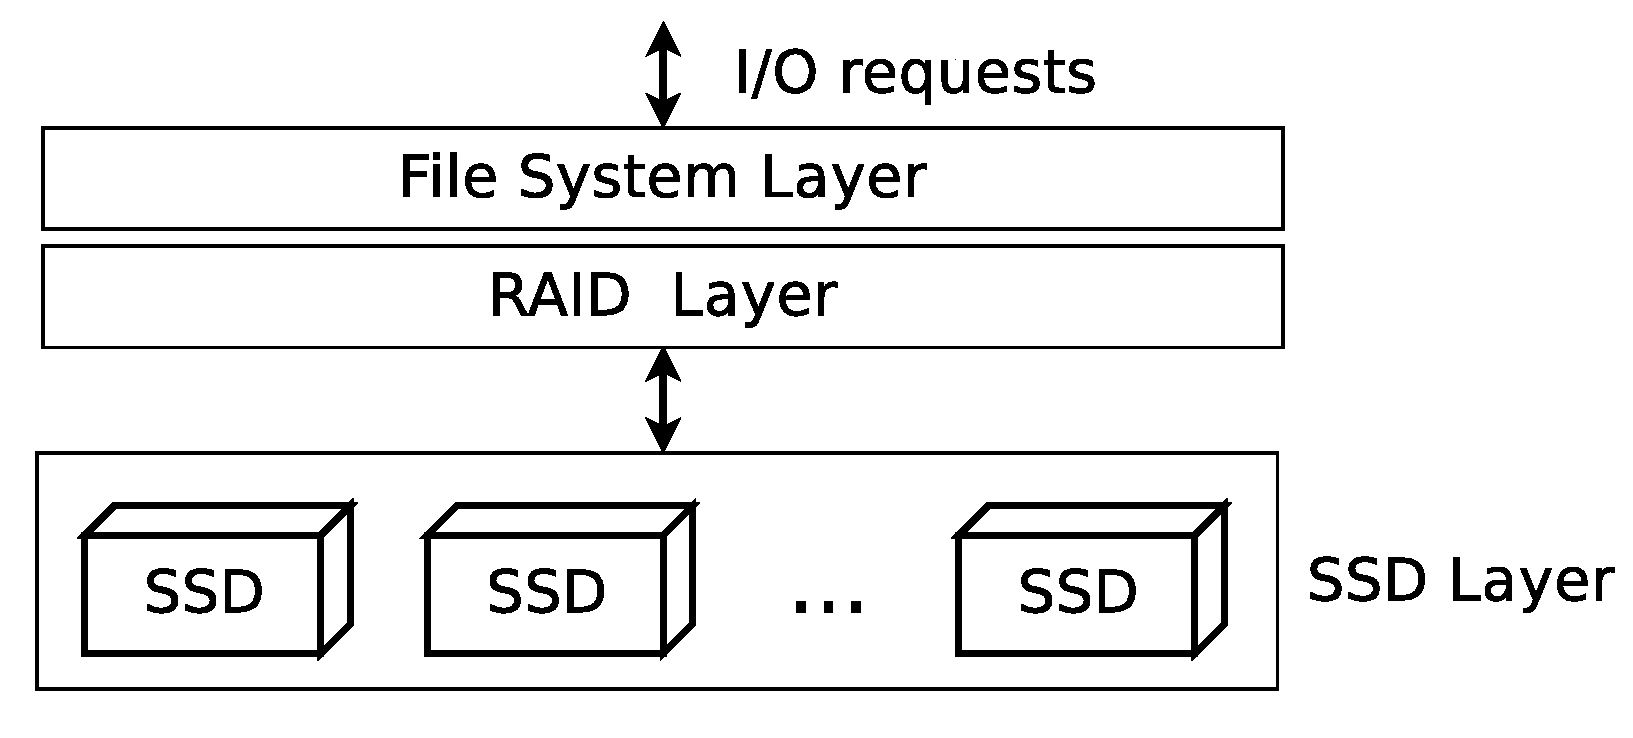
\includegraphics[width=0.8\linewidth]{figs/typical_raid}
\caption{The SSD RAID layout considered in TWEEN.}
\label{fig:typicalraid}
\end{figure}

Small random writes are detrimental to both SSD performance
\cite{kim08,chen09,min12} and RAID performance \cite{stodolsky93}.  They exhibit
in many real-world workloads including those in online transaction-processing
(OLTP) systems \cite{wong02}, desktops \cite{harter11} and enterprise servers
\cite{kavalanekar08}. Also, modern databases and critical applications tend to
call \texttt{fsync/sync} frequently to force {\em synchronous writes}, which
cause writes to be relatively small and random \cite{harter11}.
	   
%partial-stripe writes frequently.  Moreover, recent studies show that random
%writes commonly occur in both enterprise \cite{chan14} and desktop
%\cite{harter11} workloads.  Also, 
	
This section considers two specific types of small random writes that can happen
in an SSD RAID, namely {\em partial-block writes} and {\em partial-stripe
    writes}, whose request sizes are too small and do not align with the
granularities of the SSD and RAID operations, respectively. We collectively call
them {\em partial writes}, which incur performance overhead to SSD RAID as
described below.  Figure~\ref{fig:typicalraid} shows the SSD RAID layout that we
consider in TWEEN.

%\subsection{Partial-Block Writes} 

%Partial writes introduce performance overhead to an SSD RAID.  We classify
%partial writes into \textit{partial-stripe writes} in RAID and
%\textit{partial-block updates} in SSDs. In RAID, partial-stripe writes refer to
%writes that cover only part of a stripe. While these writes are handled using
%either read-modify write or reconstruct write in a parity-based RAID, both
%require extra read operations for maintaining parity consistency.  In SSDs,
%\textit{partial-block updates} refer to writes that change a portion of pages
%in a block. Partial-block updates hinder garbage collection performance and
%shorten the lifetime of SSDs as they tend to fragment a block with live and
%stale pages.

%Figure~\ref{fig:typicalraid} shows a typical SSD RAID setup.  Partial writes
%can occur in either (or both) the (1) SSD layer and the (2) RAID layer.  Our
%goal is to eliminate both partial-stripe writes and partial-block updates
%\textit{on the write path} to achieve optimal update performance and enhance
%SSD lifetime.  
%In this section, we separately study the causes and impacts of the two kinds
%of partial writes and propose a novel file system layer that couples NVRAM
%with a log-structured design as solution.

%\paragraph{When do they happen} 

\subsection{Partial-Block Writes}

In the SSD layer, partial-block writes are the writes that update only a
portion of pages in an SSD block.  Because of out-of-place writes in SSDs
\cite{agrawal08}, 
partial-block writes eventually cause SSD blocks to
contain a mix of live and stale pages, leading to internal fragmentation
\cite{chen09}.  Such internal fragmentation increases the write amplification
overhead of garbage collection, because each time garbage collection needs to
copy many live pages from the chosen block to a free block. If the number of
stale pages in a block is small, then live pages of multiple blocks need to be
relocated so as to reclaim a block that is full of clean pages. Note that the
large write amplification overhead is seen regardless of the underlying
address mapping schemes in FTL \cite{min12}. 

%In an SSD RAID, we see that partial-block updates occur if the RAID layer
%issues write requests that are either (1) unaligned to block boundaries or
%(2) having write size smaller than a block. Typically, the SSD controller
%handles partial-block updates by writing the new data to a clean block and
%marking the original pages as \textit{stale}.

%\paragraph{Why are they harmful} 

%The impacts of partial-block updates are two-fold. First, modern SSDs adopt
%interleaving techniques to boost I/O performance. Large writes spanning across
%multiple pages are inherently faster than small writes. Writes in
%multiples of the \textit{clustered page} \cite{kim12toc} size achieve better 
%I/O performance as they can write to multiple NAND flash chips in parallel.

%\red{[write size vs throughput experiment]}

%However, the fragmentation of live and stale pages in blocks eventually leads
%to write amplification. For page-level mapping FTLs, garbage collection
%suffers from large copying overhead as the controller needs to migrate live
%pages from the victim block to another clean block. For hybrid mapping FTLs,
%garbage collection is likely to trigger the expensive \textit{full merge}
%\cite{gupta09} which copies live pages from both the log blocks and data
%blocks. In either case, write amplification occurs as a result of the
%NAND flash chips receiving extra page writes due to partial-block
%updates.

%\red{[write amplification experiment]} \\

%\paragraph{Solution} 

%One intuitive approach to eliminate partial-block updates is to let the RAID
%layer align writes to the SSD block boundary before issuing them.  For
%page-level mapping FTLs, this eliminates copying overhead in garbage
%collection as all pages in a SSD block are either stale or live.  For hybrid
%mapping FTLs, garbage collection becomes a series of efficient \textit{switch
%merge} \cite{gupta09} operations since one can just replace a data block
%of stale pages with its corresponding log block.  However, the alignment
%operation is costly because it often enlarges the write size by first
%reading data to pack the unaligned writes.

\subsection{Partial-Stripe Writes}

%\paragraph{When do they happen} 

Partial-stripe writes are the writes whose request sizes are smaller than the
size of a stripe in RAID.  Depending on the write size, RAID handles a 
partial-stripe write based on one of the two approaches \cite{chen95}: (1)
\textit{read-modify write} and (2) \textit{reconstruct write} (see
Section~\ref{sec:parity_background}).  Both
reconstruct writes and read-modify writes are inferior in performance as they
incur extra reads before writes.  Instead, it is more desirable to issue 
{\em full-stripe writes}, which incur no read by updating all chunks in a stripe 
and are the most efficient type of writes in RAID \cite{chen95}. 

%Typically, workloads dominated by small and random writes such as those from
%online transaction-processing (OLTP) systems \cite{wong02} tend to trigger
%partial-stripe writes frequently.  Moreover, recent studies show that random
%writes commonly occur in both enterprise \cite{chan14} and desktop
%\cite{harter11} workloads.  Also, modern databases and critical applications
%tend to call \texttt{fsync/sync} frequently to force writes to disk, which
%cause writes to be relatively small and random \cite{harter11}.

%\paragraph{Why are they harmful} 

%\paragraph{Solution} 

%However, while this improves user experience, it only delays does not work well
%under intensive workload once the NVRAM is exhausted \red{[CITE]}.

%Intuitively, a log-based design converts small random writes to large
%sequential writes through batching. Updates are packed in a log until there
%are sufficient data to issue a full-stripe write~\cite{menon95}.  Although a
%log-based design eliminates read operations on the write path, the garbage
%collection mechanism requires careful consideration as it is known to hinder
%system performance~\cite{seltzer95}.

